%%%%%%%%%%%%%%%%%%%%%%%%%%%%%%%%%%%%%%%%%%%%%%%%%%%%%%%%%%%%%%%%%%%%%%%%%%%%%%%%%%%%%
% Model Predictive Control
%
%
%
%
%%%%%%%%%%%%%%%%%%%%%%%%%%%%%%%%%%%%%%%%%%%%%%%%%%%%%%%%%%%%%%%%%%%%%%%%%%%%%%%%%%%

\section{Model Predictive Control}

Compared to all topics in process control, the concepts of model predictive control (MPC) is perhaps the closest resemblance to modern RL.  MPC is a model-based control strategy (known as a planning method in RL literature) that optimizes the input trajectory of a system by using the functional equation (a function where the unknowns are also functions) generated from the system's state information together with a value function. The performance of MPCs heavily relies on the accuracy of system identification as the input trajectory is solved by extremizing an objective function using mathematical programming (MP) as a function of the process model \cite{mpc}. The objective function is typically given as:
\begin{equation}
    J = \sum\limits^{N}_{i = 1} x_i^TQx_i + \sum\limits^N_{i=1}u_i^TRu_i
    \label{eq:mpc_cost}
\end{equation}
where $N$, $Q$, and $R$ are the prediction horizon and tuning matrices, respectively. Superscript $T$ denotes the transpose operation. $Q$ and $R$ are diagonal matrices and are used to emphasize importance on different state and inputs, respectively. Here, $x$ and $u$ are given as:
\begin{equation}
    x_{sp} - x_i
\end{equation}
\begin{equation}
    u_{ss} - u_i
\end{equation}
where subscripts $sp$ and $ss$ denote the set-point and steady state, respectively. Often times, MPCs are applied onto integrating processes; thus, using $\Delta u$ to handle such scenarios.

Implementation-wise, MPC uses a receding horizon approach where the controller predicts and optimizes for a set amount of steps into the future.  However, only the first control action is implemented.  During the next sampling time, the trajectory is re-optimized and the cycle repeats. The length of the input trajectory and the number of steps the controller predicts into the future are known as the control and prediction horizon, respectively. During design, it is paramount to ensure that both the prediction and control horizons are adequate in length to ensure optimal dynamic performance.  Intuitively, the prediction and control horizon can be related to the everyday task of driving a car.  It would be very dangerous if we only consider events one second into the future because it would be difficult to react to curves and other road side disturbances; therefore, the prediction and control horizons must be sufficiently long to ensure safe and optimal driving practices. Typically, the control horizon is chosen to be shorter than the prediction horizon due to computational cost and the unimportance of unnecessarily long input trajectories \cite{prediction_horizon}.  One flaw with the receding horizon approach is its extremely expensive online computational cost, especially in large non-linear systems.  

Explicit MPC was developed to mitigate this computational burden by leveraging parametric programming to pre-compute solutions to the optimization problem offline \cite{explicit_MPC}.  During online evaluation, the controller simply looks up the optimal input from a dictionary of pre-computed solutions, making online evaluation extremely fast. This idea is exactly equivalent to RL, where the agent is trained offline (i.e., solves the optimal policies offline), allowing extremely fast online evaluations. 

Ultimately, MPCs provide many advantages compared to classical control strategies.  For example, MPC considers long term planning and identifies the optimal input trajectory rather than the best immediate action.  Furthermore, MPCs have predictive capabilities and can anticipate future events, allowing the controller to plan future control actions accordingly.  A third advantage is that the MP methods used in MPC have been widely demonstrated to handle both input and state constraints relatively successfully.  In modern times, MPCs are often implemented in the supervisory control layer.

The process control hierarchy is shown in Figure \ref{fig:rto_mpc_pid}. Starting from the bottom, the \textit{regulatory controllers} are typically used to ensure regulation of disturbances and set-point tracking of the process and directly actuate the process instrumentation.  A common regulatory controller is the Proportional-Integral-Derivative controller (PID). The layers above are known as the \textit{supervisory controllers}. MPC is a common supervisory controller and is classically implemented for regulation or set-point tracking problems exclusively.  Economic objectives of the process were managed by the real time optimization (RTO) layer through steady state optimization \cite{rto}. More recently, control practitioners began to unify the ideas of RTO and MPC into a centralized algorithm called economic model predictive control (EMPC).  Here, the economic objective of the RTO is placed into the objective function of the MPC, allowing for the input trajectory to optimize the economic objective instead \cite{empc2, empc1}. 

\begin{figure}[H]
    \centering
    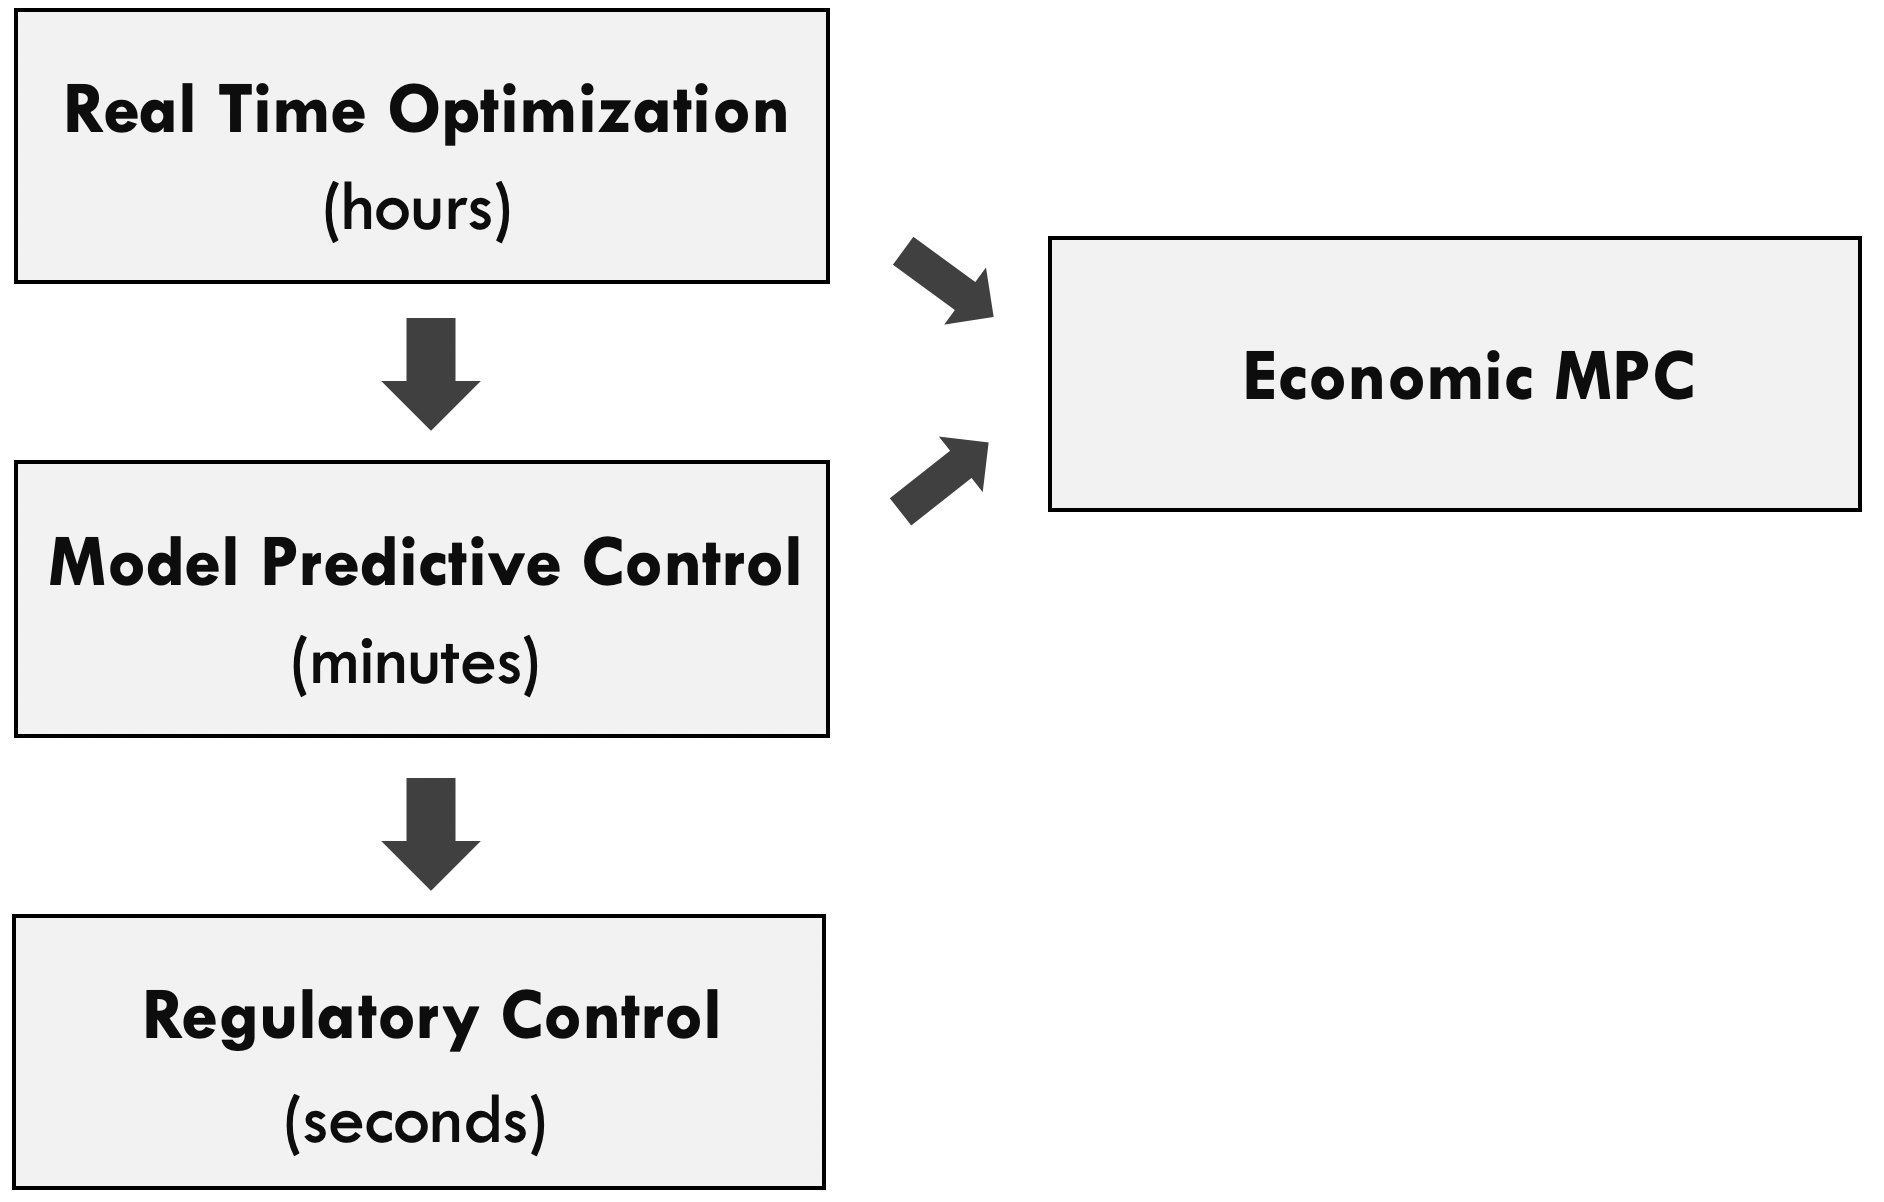
\includegraphics[width=0.5\textwidth]{images/ch1/rto_mpc_pid.jpeg}
    \caption{A typical industrial control architecture.}
    \label{fig:rto_mpc_pid}
\end{figure}

Comparatively, RL can be described as a general control algorithm and can be used to replace \textit{any} layer in Figure \ref{fig:rto_mpc_pid}. For example, a MPC or PID based RL would have its reward function to be identical as the negative of Equation \ref{eq:mpc_cost}.  In the EMPC case, the reward function of RL would instead be the economic objective.  In Chapter 4, the performance of RL based supervisory controls will be extensively compared to traditional methods on simple and complicated processes. Additionally, the pros and cons of each method will be summarized.